\documentclass[a4paper]{article}
\usepackage[margin=1cm]{geometry}
\usepackage{amsmath, amssymb}
\usepackage{graphicx}
\usepackage{tikz}
\usetikzlibrary{arrows.meta}
\pagestyle{empty}

\definecolor{c0}{HTML}{E53935}
\definecolor{c1}{HTML}{1E88E5}
\definecolor{c2}{HTML}{43A047}
\definecolor{c3}{HTML}{FB8C00}
\definecolor{c4}{HTML}{8E24AA}
\definecolor{c5}{HTML}{00ACC1}
\definecolor{c6}{HTML}{F4511E}
\definecolor{c7}{HTML}{3949AB}
\definecolor{c8}{HTML}{7CB342}
\definecolor{c9}{HTML}{C2185B}
\definecolor{c10}{HTML}{FF7043}
\definecolor{c11}{HTML}{26A69A}
\definecolor{c12}{HTML}{5C6BC0}
\definecolor{c13}{HTML}{FFCA28}
\definecolor{c14}{HTML}{AB47BC}

\begin{document}

\begin{center}
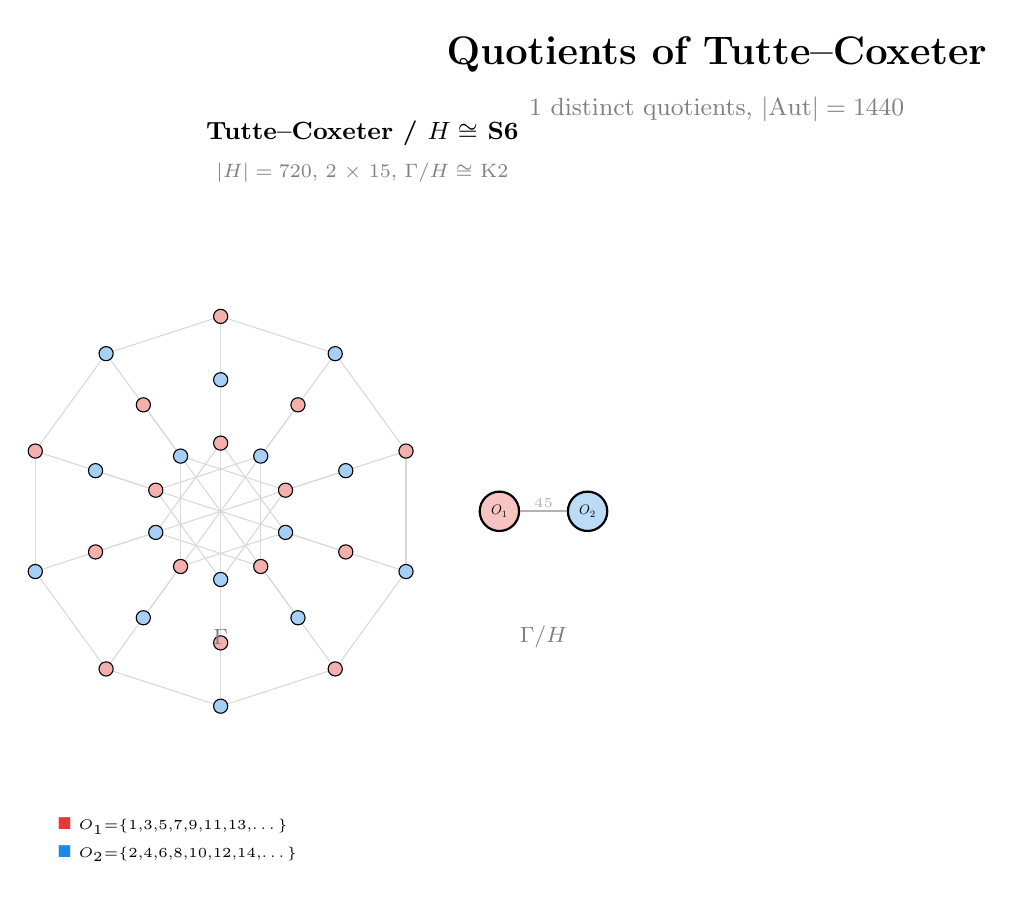
\begin{tikzpicture}[
  ov/.style={circle, draw, semithick, minimum size=3.5mm, inner sep=0pt},
  ovs/.style={circle, draw, thin, minimum size=1.8mm, inner sep=0pt},
  qv/.style={circle, draw, thick, minimum size=5mm, inner sep=0pt},
  cardtitle/.style={font=\small\bfseries},
  cardsub/.style={font=\scriptsize, text=gray},
  glabel/.style={font=\footnotesize, text=gray},
]
\node[font=\Large\bfseries] at (0, 11.5) {Quotients of Tutte--Coxeter};
\node[font=\small, text=gray] at (0, 10.8) {1 distinct quotients, $|\mathrm{Aut}|=1440$};

% Card 1: H=S6
\node[cardtitle] at (-4.50,10.50) {Tutte--Coxeter / $H \cong$ S6};
\node[cardsub] at (-4.50,10.00) {$|H|=720$, 2 $\times$ 15, $\Gamma/H \cong$ K2};
\draw[gray!30, thin] (-6.300,8.175) -- (-7.755,7.702);
\draw[gray!30, thin] (-6.300,8.175) -- (-6.300,7.371);
\draw[gray!30, thin] (-6.300,8.175) -- (-4.845,7.702);
\draw[gray!30, thin] (-7.755,7.702) -- (-8.654,6.465);
\draw[gray!30, thin] (-7.755,7.702) -- (-7.282,7.052);
\draw[gray!30, thin] (-8.654,6.465) -- (-8.654,4.935);
\draw[gray!30, thin] (-8.654,6.465) -- (-7.889,6.216);
\draw[gray!30, thin] (-8.654,4.935) -- (-7.755,3.698);
\draw[gray!30, thin] (-8.654,4.935) -- (-7.889,5.184);
\draw[gray!30, thin] (-7.755,3.698) -- (-6.300,3.225);
\draw[gray!30, thin] (-7.755,3.698) -- (-7.282,4.348);
\draw[gray!30, thin] (-6.300,3.225) -- (-4.845,3.698);
\draw[gray!30, thin] (-6.300,3.225) -- (-6.300,4.029);
\draw[gray!30, thin] (-4.845,3.698) -- (-3.946,4.935);
\draw[gray!30, thin] (-4.845,3.698) -- (-5.318,4.348);
\draw[gray!30, thin] (-3.946,4.935) -- (-4.711,5.184);
\draw[gray!30, thin] (-3.946,4.935) -- (-3.946,6.465);
\draw[gray!30, thin] (-4.711,5.184) -- (-7.889,6.216);
\draw[gray!30, thin] (-4.711,5.184) -- (-5.476,5.432);
\draw[gray!30, thin] (-7.889,6.216) -- (-7.124,5.968);
\draw[gray!30, thin] (-7.124,5.968) -- (-5.791,6.401);
\draw[gray!30, thin] (-7.124,5.968) -- (-6.300,4.834);
\draw[gray!30, thin] (-5.791,6.401) -- (-5.318,7.052);
\draw[gray!30, thin] (-5.791,6.401) -- (-5.791,4.999);
\draw[gray!30, thin] (-5.318,7.052) -- (-7.282,4.348);
\draw[gray!30, thin] (-5.318,7.052) -- (-4.845,7.702);
\draw[gray!30, thin] (-7.282,4.348) -- (-6.809,4.999);
\draw[gray!30, thin] (-6.809,4.999) -- (-5.476,5.432);
\draw[gray!30, thin] (-6.809,4.999) -- (-6.809,6.401);
\draw[gray!30, thin] (-5.476,5.432) -- (-6.300,6.566);
\draw[gray!30, thin] (-6.300,6.566) -- (-6.300,7.371);
\draw[gray!30, thin] (-6.300,6.566) -- (-7.124,5.432);
\draw[gray!30, thin] (-6.300,7.371) -- (-6.300,4.029);
\draw[gray!30, thin] (-6.300,4.029) -- (-6.300,4.834);
\draw[gray!30, thin] (-6.300,4.834) -- (-5.476,5.968);
\draw[gray!30, thin] (-5.476,5.968) -- (-6.809,6.401);
\draw[gray!30, thin] (-5.476,5.968) -- (-4.711,6.216);
\draw[gray!30, thin] (-6.809,6.401) -- (-7.282,7.052);
\draw[gray!30, thin] (-7.282,7.052) -- (-5.318,4.348);
\draw[gray!30, thin] (-5.318,4.348) -- (-5.791,4.999);
\draw[gray!30, thin] (-5.791,4.999) -- (-7.124,5.432);
\draw[gray!30, thin] (-7.124,5.432) -- (-7.889,5.184);
\draw[gray!30, thin] (-7.889,5.184) -- (-4.711,6.216);
\draw[gray!30, thin] (-4.711,6.216) -- (-3.946,6.465);
\draw[gray!30, thin] (-3.946,6.465) -- (-4.845,7.702);
\node[ovs, fill=c0!40] at (-6.300,8.175) {};
\node[ovs, fill=c1!40] at (-7.755,7.702) {};
\node[ovs, fill=c0!40] at (-8.654,6.465) {};
\node[ovs, fill=c1!40] at (-8.654,4.935) {};
\node[ovs, fill=c0!40] at (-7.755,3.698) {};
\node[ovs, fill=c1!40] at (-6.300,3.225) {};
\node[ovs, fill=c0!40] at (-4.845,3.698) {};
\node[ovs, fill=c1!40] at (-3.946,4.935) {};
\node[ovs, fill=c0!40] at (-4.711,5.184) {};
\node[ovs, fill=c1!40] at (-7.889,6.216) {};
\node[ovs, fill=c0!40] at (-7.124,5.968) {};
\node[ovs, fill=c1!40] at (-5.791,6.401) {};
\node[ovs, fill=c0!40] at (-5.318,7.052) {};
\node[ovs, fill=c1!40] at (-7.282,4.348) {};
\node[ovs, fill=c0!40] at (-6.809,4.999) {};
\node[ovs, fill=c1!40] at (-5.476,5.432) {};
\node[ovs, fill=c0!40] at (-6.300,6.566) {};
\node[ovs, fill=c1!40] at (-6.300,7.371) {};
\node[ovs, fill=c0!40] at (-6.300,4.029) {};
\node[ovs, fill=c1!40] at (-6.300,4.834) {};
\node[ovs, fill=c0!40] at (-5.476,5.968) {};
\node[ovs, fill=c1!40] at (-6.809,6.401) {};
\node[ovs, fill=c0!40] at (-7.282,7.052) {};
\node[ovs, fill=c1!40] at (-5.318,4.348) {};
\node[ovs, fill=c0!40] at (-5.791,4.999) {};
\node[ovs, fill=c1!40] at (-7.124,5.432) {};
\node[ovs, fill=c0!40] at (-7.889,5.184) {};
\node[ovs, fill=c1!40] at (-4.711,6.216) {};
\node[ovs, fill=c0!40] at (-3.946,6.465) {};
\node[ovs, fill=c1!40] at (-4.845,7.702) {};
\node[glabel] at (-6.30,4.10) {$\Gamma$};
\node[qv, fill=c0!30] (c0o0) at (-2.760,5.700) {\scalebox{0.5}{$O_{1}$}};
\node[qv, fill=c1!30] (c0o1) at (-1.640,5.700) {\scalebox{0.5}{$O_{2}$}};
\draw[gray!60, thick] (c0o0) -- node[font=\tiny, auto, inner sep=1pt] {45} (c0o1);
\node[glabel] at (-2.20,4.10) {$\Gamma/H$};
\node[anchor=west, font=\tiny] at (-8.50,1.70) {\textcolor{c0}{$\blacksquare$} $O_{1}$=\{1,3,5,7,9,11,13,\ldots\}};
\node[anchor=west, font=\tiny] at (-8.50,1.35) {\textcolor{c1}{$\blacksquare$} $O_{2}$=\{2,4,6,8,10,12,14,\ldots\}};
\end{tikzpicture}
\end{center}

\end{document}